\chapter{Design}

Il presente capitolo descrive le scelte architetturali, tecnologiche e progettuali adottate per soddisfare gli obiettivi e i requisiti definiti nel capitolo precedente. L'attenzione si concentra sulle funzionalità sviluppate o analizzate durante il tirocinio, pur accennando alle linee guida per alcune delle funzionalità future, al fine di offrire una visione più completa del sistema.

La progettazione del nuovo sistema punta a superare i limiti identificati nel legacy, adottando un'architettura moderna, modulare e scalabile, che semplifichi la gestione e consenta l'integrazione di nuove funzionalità. Particolare attenzione è stata dedicata alla separazione delle responsabilità tra i vari componenti, alla retrocompatibilità con il sistema attuale e al miglioramento dell'esperienza utente.

Il capitolo è strutturato come segue: dopo una descrizione dell’architettura generale del sistema, si approfondiranno le principali componenti e funzionalità chiave, come la multiutenza e la gestione dei template. Infine, saranno discussi gli aspetti relativi al miglioramento del database e alle strategie messe in campo per garantire la corretta coesione tra i due sistemi.

\section{Architettura generale}

Per la progettazione del nuovo sistema è stata adottata un'architettura a microservizi, caratterizzata da una separazione netta tra frontend e backend. Questa scelta è motivata dalla necessità di superare i limiti architetturali del sistema legacy, introducendo modularità e una chiara separazione delle responsabilità tra i vari componenti.

Nel nuovo sistema, il frontend è rappresentato da un singolo microservizio dedicato alla logica di presentazione dei dati e all'interazione con l'utente. Il backend, invece, è stato suddiviso in molteplici microservizi indipendenti, ciascuno dedicato a un modulo o a una funzionalità specifica dell'applicativo. Questa scomposizione consente di ottenere una maggiore flessibilità, facilitando sia l'aggiunta di nuove funzionalità che la manutenzione del sistema.

I microservizi comunicano tra loro utilizzando il protocollo HTTP e, più specificamente, attraverso API RESTful che ciascuno di essi espone. Queste API vengono inoltre utilizzate sia dal frontend sia per la creazione delle API pubbliche aziendali. Queste ultime, già presenti insieme al sistema legacy, sono state rinnovate per adattarsi alle nuove logiche di funzionamento introdotte nel nuovo sistema.

\subsection{Frontend}
Il frontend è stato progettato come una Single-Page Application (SPA) utilizzando il framework Next.js\footnote{\url{https://nextjs.org}}, scelta che consente di offrire agli utenti un'esperienza fluida ed un accesso rapido da qualsiasi browser, senza bisogno di installare nessun applicativo. Questo microservizio si occupa esclusivamente della logica di presentazione, implementando l'interfaccia grafica e gestendo l'interazione con gli utenti finali.

L'architettura del frontend segue un approccio modulare, in cui ogni pagina e componente è organizzato in base a un sistema di routing gerarchico, denominato App Router\footnote{\url{https://nextjs.org/docs/app}} e facente parte di Next.js. Grazie a tale sistema di routing, la struttura delle cartelle rispecchia direttamente quella degli URL, permettendo una gestione chiara e intuitiva delle varie sezioni dell’applicazione.

Per velocizzare lo sviluppo dell'interfaccia e garantire un design coerente, è stato adottato il template TailAdmin\footnote{\url{https://tailadmin.com}}, una libreria di componenti predefiniti completamente personalizzabili. Questo ha permesso di ridurre il tempo di sviluppo mantenendo comunque la possibilità di adattare l’interfaccia grafica alle esigenze specifiche del progetto. Il template fornisce inoltre pagine già strutturate, che sono state opportunamente modificate per integrarsi con la logica applicativa del sistema.

Un altro aspetto chiave dell'architettura è la gestione dell'autenticazione, implementata tramite la libreria dedicata \texttt{next-auth}\footnote{\url{https://authjs.dev}}. Sebbene Next.js offra la possibilità di definire API direttamente all'interno del frontend, si è scelto di non utilizzare questa funzionalità per la gestione dell'autenticazione. Invece, tale processo è stato demandato a un microservizio che risiede nel backend del sistema, responsabile di tutto ciò che riguarda autenticazione ed autorizzazione.

Anche tutte le operazioni di elaborazione dei dati, come le computazioni o la gestione delle regole di business, sono demandate al backend. Questo approccio garantisce una maggiore coerenza e centralizzazione della logica applicativa, riducendo la complessità del frontend e migliorando la scalabilità del sistema.

\subsection{Backend}
Come già accennato, il backend non è stato concepito come un unico servizio monolitico, ma si è optato per una suddivisione in più microservizi, ciascuno responsabile di una specifica funzionalità o modulo del sistema. La definizione di questi microservizi è stata guidata dall'analisi del dominio (\Cref{sec:domain-analysis}), individuando le principali entità e le loro responsabilità all'interno dell'architettura complessiva. Questo approccio ha permesso di modellare il backend in modo coerente con le esigenze del sistema, garantendo una chiara separazione delle responsabilità e facilitando l'evoluzione futura della piattaforma.

Di seguito, vengono descritti i principali microservizi di cui il backend è composto.

\paragraph{Auth}
Il microservizio \texttt{auth} è responsabile dell'autenticazione e dell'autorizzazione degli utenti. L'autenticazione è implementata attraverso il meccanismo JWT (JSON Web Token), che consente di gestire sessioni sicure senza la necessità di mantenere uno stato lato server.
L'autorizzazione, invece, fornisce un sistema per determinare se un utente ha i permessi necessari per eseguire una determinata azione. Questa valutazione si basa sul ruolo dell'utente e sulla licenza a lui associata, garantendo così un controllo granulare sugli accessi alle funzionalità della piattaforma.

\paragraph{Report}
Il microservizio \texttt{report} gestisce la generazione e la visualizzazione dei report relativi alle attività di filtraggio DNS. Nella prima versione del sistema, questa funzionalità è limitata alla visualizzazione di report specifici per gli MSP. Questo microservizio si interfaccia con il database per raccogliere e aggregare i dati necessari, fornendo agli utenti una panoramica dettagliata sull'attività di filtraggio e sull'efficacia delle policy applicate.

\paragraph{Organization}
Il microservizio \texttt{organization} è un componente chiave per l'implementazione della multiutenza. Esso si occupa di gestire tutte le operazioni CRUD sugli utenti, consentendo di creare nuovi account, modificare i ruoli, nonché rimuovere utenti dalle organizzazioni.
Grazie a questo servizio, più utenti possono essere associati a un'unica organizzazione con livelli di accesso differenziati, migliorando la flessibilità e la gestione delle autorizzazioni.

\paragraph{Protection}
Il microservizio \texttt{protection} è responsabile della gestione delle policy di protezione applicate agli utenti e alle organizzazioni. Questo servizio permette di creare, modificare ed eliminare i profili di protezione, ossia insiemi di regole che determinano quali contenuti possono essere filtrati o consentiti.
Inoltre, gestisce la creazione e l’amministrazione dei profili condivisi, che consentono di applicare una configurazione comune a più clienti senza dover definire manualmente le stesse regole per ciascuno di essi.

\paragraph{Licensing}
Il microservizio \texttt{licensing} si occupa della gestione delle licenze associate agli utenti e alle organizzazioni. Attraverso questo servizio, è possibile visualizzare lo stato delle licenze attive, gestire le assegnazioni e monitorare la loro scadenza.
Questo microservizio è essenziale per garantire che ogni utente abbia accesso solo alle funzionalità previste dal proprio piano, permettendo un controllo efficace sui livelli di servizio offerti.

\subsubsection{Architettura a livelli}
Tutti i microservizi appena discussi seguono un'architettura uniforme, basata sull'esposizione di API REST da parte del framework Web Express\footnote{\url{https://expressjs.com}}. Questa standardizzazione semplifica lo sviluppo e la manutenzione, garantendo che i microservizi siano facilmente scalabili e sostituibili senza impattare il funzionamento complessivo del sistema. Dal punto di vista strutturale, ogni microservizio è organizzato secondo un'architettura a livelli, ben visibile in \Cref{fig:microservice-architecture}, e composta dalle seguenti componenti:

\begin{itemize}
  \item \textbf{Routes}: rappresentano il punto di ingresso delle richieste HTTP. Si occupano di instradare ogni richiesta in base al percorso e al metodo HTTP associato, inoltrandola al controller appropriato per la gestione.

  \item \textbf{Controllers}: gestiscono le richieste ricevute, validano i parametri in ingresso ed eseguono le operazioni necessarie delegando l’elaborazione al livello dei servizi. Una volta ottenuto il risultato, i controller generano le risposte HTTP da restituire ai client.

  \item \textbf{Services}: costituiscono il livello dedicato all'implementazione della logica di business. Si occupano di elaborare i dati e interagire con il livello di accesso agli stessi, senza dipendere direttamente dalle richieste HTTP. Questo livello intermedio garantisce una maggiore modularità e facilita il riutilizzo delle funzionalità tra diversi controller.

  \item \textbf{Repositories}: forniscono un’interfaccia per l’accesso ai dati, eseguendo operazioni di lettura e scrittura sul database. Questo livello è responsabile esclusivamente della gestione dei dati e dell'interazione con il database, mantenendo separata la logica applicativa dal livello di persistenza.
\end{itemize}

\begin{figure}
  \centering
  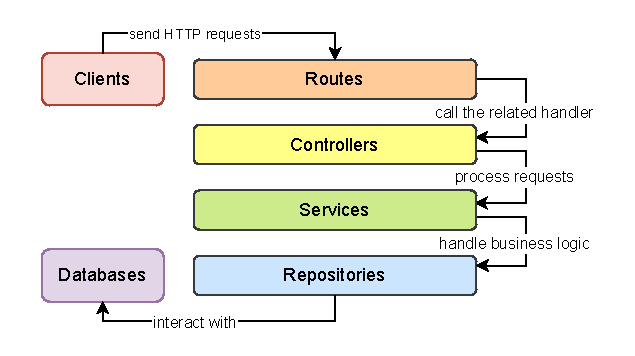
\includegraphics[width=0.9\textwidth]{figures/microservice-architecture.pdf}
  \caption{Architettura a livelli dei microservizi del backend}
  \label{fig:microservice-architecture}
\end{figure}

Questa suddivisione in livelli garantisce una chiara separazione delle responsabilità, migliorando la manutenibilità e la scalabilità del sistema. Inoltre, consente di evolvere il backend in modo strutturato, rendendo più semplice l'aggiunta di nuove funzionalità o modifiche alle logiche applicative senza impattare gli altri componenti.
